Eine der besten Möglichkeiten, Temperaturen zu messen, ist die Infrarottechnik.
Sie bietet einige erhebliche Vorteile, durch die Fähigkeit zur berührungslosen
Temperaturmessung. Zum einen wird der zu messende Gegenstand in keinerlei Weise
beeinflusst, was zum Beispiel die Gefahr der physischem Zerstörung, durch
Berühren empfindlicher Gegenstände, wie Blätter verhindert.(Abbildung
\ref{fig:infrarot_pflanze}) Die Entfernung zum Messpunkt ermöglicht auch, sehr
hohe Temperaturen zu messen, ohne die Infrarotsensorik durch zu hohe
Temperaturen zu gefährden. \begin{figure}[!h]
	\centering
	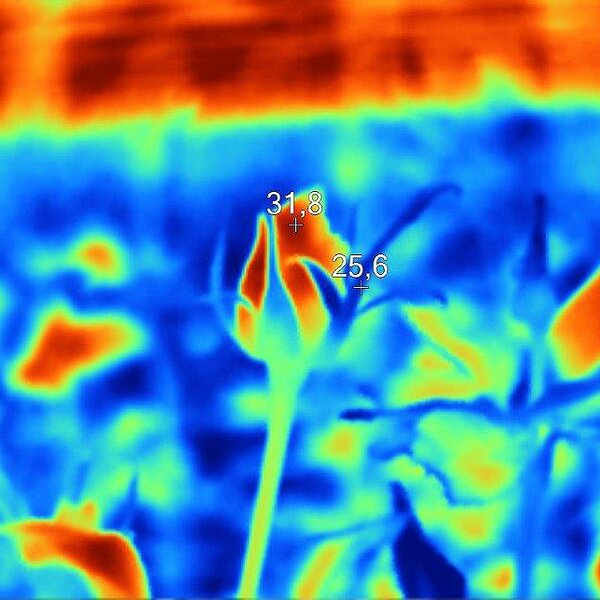
\includegraphics[width=0.7\textwidth]{bilder/Measuring-crop-temperatures .jpeg}
	\caption[Infrarotaufnahme einer Pflanze]{Infrarotaufnahme einer Pflanze\cite{IRPflanze}}
	\label{fig:infrarot_pflanze}
\end{figure}

Die Bestandteile einer Infrarotkamera beinhalten eine Optik, einen Detektor,
sowie die Verarbeitungselektronik. (Abbildung \ref{fig:aufbau infrarotsensor})
\begin{figure}[ht]
	\centering
	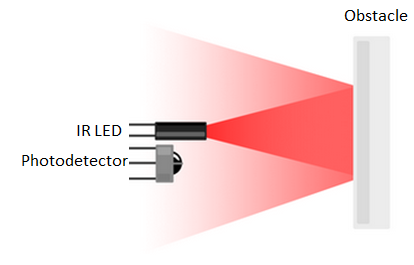
\includegraphics[width=0.7\textwidth]{bilder/infrarotsensor.png}
	\caption[Aufbau eines IR-Messgeräts]{Aufbau eines IR-Messgeräts\cite{IR}}
	\label{fig:aufbau infrarotsensor}
\end{figure}

Die Optiken sind häufig Linsen aus Germanium, da diese transparent für Infrarotlicht sind. Es
gibt zwei Gruppen von Detektoren. Thermische Detektoren (Bolometer und
thermophile Detektoren) besitzen sensitive Flächen, welche von der Energie der
infraroten Strahlung erwärmt werden. Sie sind genau und reagieren schnell,
zudem arbeiten thermische Detektoren bei Raumtemperatur, es wird also keine
zusätzliche Kühlelektronik benötigt. Wenn es eine noch höhere
Temperaturempfindlichkeit benötigt, wobei man von $<$20 mK spricht, werden
Quantendetektoren. Jedoch müssen diese gekühlt werden, da sie sonst ein hohes
Eigenrauschen aufweisen.\cite{may2015transiente}

Funktionsweise von Infrarotthermographie: \\ Messgegenstände mit einer
Temperatur von $>$ 900K strahlen Energie ab, der in mithilfe von
Wärmebildtechnik sichtbar gemacht werden kann und so als Bild, für den Menschen
sichtbar dargestellt werden kann. Hierzu werden die Spektralbereiche
Nahinfrarot(NIR), mittleres Infrarot (MIR) und langes Infrarot (LIR)
betrachtet. Diese Spektren teilen sich in drei Teile im Bereich von 780 bis
1400nm auf.\cite{schuster2004infrarotthermographie}